\section{Введение}

Модель случайных блужданий без самопересечений (далее - СБС) - одна из наиболее широко изученных моделей из класса линейных полимеров. 
Более того, она является одной из простейших моделей для изучения критического поведения - так, в случае когда модель усложнена наличием взаимодействия между ближайшими узлами цепочки, её фазовый переход оказывается зафиксирован между состояниями её растворителя, и при термическом равновесии системы полученная полимерная цепочка будет схлопнутой в условиях сильного растворителя или вытянутой в слабом растворителе.
Трикритичность данного перехода была описана в работе \cite{Gennes1979}.

Влияние близких связей было широко рассмотрено среди класса моделей магнитного полимера, взаимодействие между узлами которых стало ещё более сложным:
каждый узел обладает спином, а сила взаимодействия между ближайшими узлами стала отдельным параметром. 
Её название - модель Изинга на случайном блуждании без самопересечений.
В работе \cite{Garel1999} был рассмотрен случай, когда она так же обладает переменным внешним полем, и все заключения о её магнитных свойствах были оценены в сравнении с моделью среднего поля.
В то же время влияние геометрических свойств модели на магнитные не до конца ясно и их изучение в некоторых случаях требует статистического подхода.

В предыдущей работе \cite{faizullina2021critical} было определено, что фазовый переход двумерной модели Изинга на CБС
имеет непрерывный характер. 
В этой работе мы продолжаем изучать геометрические свойства данной модели и сравнивать их с её родительскими моделями или модификациями, такими как классическая модель Изинга на регулярной решётке, опредёленная в работе \cite{selke2006critical}, и взаимодействующее случайное блуждание без самопересечений в соответствующих критических областях. 
Мы предполагаем, что модели с похожими геометрическими свойствами будут так же иметь схожесть в магнитных, что мы рассмотрим при сравнении кумулянтов биндера в области $\theta$-перехода моделей при равных значениях асферичности.
Также могут быть интересны для рассмотрения решётки, на которых исследуются конформации модели, как параметр задающий закон, по которому определяется существование связей между узлами в цепочке. 
Данное направление было начато в частном случае для концов случайных блужданий без самопересечений на квадратной решётке в работе \cite{owczarek2008scaling}. 
В нашей работе мы рассмотрим эти результаты с долями узлов с фиксированным количество соседей на квадратной решётке, как обобщение на внутренние узлы цепочки, а так же рассмотрим поведение данного геометрического свойства среди разных решёток в пределе бесконечной длины цепочки.  

\section{Модели и методы}
В рамках данной работы определяется несколько моделей: первой будет модель Изинга на случайном блужданий без самопересечений (далее - Ising-ISAW). Энергия системы конформации $u$ (последовательности точек на решётке, на которых размещёна цепочка) фиксированной длины N с последовательностью спинов в узлах s, принимающих значение $+1$ или $-1$, рассчитывается как сумма взаимодействий между ближайшими узлами цепочки:

\begin{equation}
\label{eq:IsISAW_ham}
E(s,u) = -J \sum_{\la i, j \ra} s_i s_j,\ \ \ \ i,j \in u, |u|=N
\end{equation}
Статическая сумма модели берётся по всем возможным последовательностяv $\{s\}$ и конформациям $u$:

\begin{equation}
Z = \sum_s \sum_u \exp{(\frac{-E}{kT})}
\end{equation}

где $T$ — температура, $k$ — постоянная Больцмана. Без потери общности можно считать $kT = 1$, тем самым оставляя J самостоятелньым параметром модели.
В первой части работы модель Ising-ISAW рассматривается только на квадратной решётке, где соседями узла можно считать мономеры, расположенные сверху, снизу, слева и справа от него.

Первая часть работы посвящена сравнению Ising-ISAW с "родительских" по отношению к ней моделей. 
С одной стороны, взаимодействующая составляющая модели берётся из классических моделей Изинга - 
в частности, мы будем рассматривать классическую модель Изинга на регулярной прямоугольной решётке (далее - прямоугольный Изинг), определеную так же в работе \cite{selke2006critical}.
В ней узлы со спинами заполняют всю решётку со стороной $L=N_x$ и отношением сторон $r=\frac{N_y}{N_x}$. Длина стороны считается как количество узлов решётки в одном ряде. 
Решётка может иметь как периодический граничные условия - когда узлы на противоположных краях решётки считаются соседними - так 
Тогда энергия системы с последовательностью спинов $s$, рассчитывается как сумма взаимодействий между ближайшими узлами по всей решётке:

\begin{equation}
E(L, r, \{s\}) = -J \sum_{\la i, j \ra} s_i s_j,\ \ \ \ i,j = (x_i, u_i), (x_j, y_j) \in [1..L] \times [1..L*r]
\end{equation}

Статическая сумма модели берётся только возможным последовательностяv ${s}$:

\begin{equation}
Z = \sum_s \exp{(\frac{-E}{kT})}
\end{equation}

В качестве сравниваемого между моделями магнитного свойства определим кумулянт Биндера (или критический кумулянт):

\begin{equation}
\label{eq:Cumulant}
U_{4} = 1 - \frac{\la m^{4} \ra}{3 (m^{2})^{2}}
\end{equation}

где $\la m^{2} \ra$  - средний квадрат удельной намагниченности, $\la m^{4} \ra$ - средная удельная намагниченность в четвертой степени. 

С другой стороны, определелим модель взаимодействующего блуждания без самопересечений (далее - ISAW) на квадратной решётке из работы \cite{caracciolo2011geometrical}.
В отличие от Ising-ISAW, узлы конформации не имеют спинов, и энергия модели рассчитывается как сумма связей переменной силы J между узлами:

\begin{equation}
E(\{u\}) = \sum_{\la i, j \ra} 1,\ \ \ i,j \in u, |u|=N
\end{equation}

\begin{equation}
Z = \sum_s \exp{(- \beta E(\{s\}))}
\end{equation}

В рамках работы \cite{caracciolo2011geometrical} исследовалось поведение геометрических свойств в критической области - в частности, асферичности конформации, показателя отличия системы узлов от круга.
Для этого определим показатели формы системы, такие как тензор вращения системы - матрица корреляции координат системы из N точек $w_i = (w_{i,\alpha}, w_{i,\beta})$:

\begin{equation}\label{eq:Ten_G2}
    Q_{N,\alpha\beta} = \frac{1}{2(N+1)^{2}} \sum^{N}_{i,k=0}(w_{i,\alpha} - w_{k, \alpha})(w_{i,\beta} - w_{k, \beta})
\end{equation}

Собственные значения $q_1, q_2$ полученного тензора вращения можно интерпретировать как квадраты длин полуосей эллипса вращения системы.
Их отношение для системы длины $N$ равна:

\begin{equation}
r = \sqrt{\frac{\la q_1 \ra_N}{\la q_2 \ra_N}}
\end{equation}

Так же эти значения используются для расчёта ещё одного показателя формы - 
средней асферичности:

\begin{equation}
\label{eq:Asphericity}
    \mathcal{A} = \left\langle \frac{(q_{1} - q_{2})^{2}}{(q_{1} + q_{2})^{2}} \right\rangle_{N}
\end{equation}

В рамках второй части работы будут рассмотрены модификации исследуемой системы Ising-ISAW, имеющие изменения в выбранной решётке, законами которой определяется "близость узлов" цепочки и координационное число - максимально возможное количество связей с одним узлом цепочки или максимальное число соседей у узла решётки:
в квадратной решётке соседями узла можно считать мономеры, расположенные сверху, снизу, слева и справа и него, 
в то время как в треугольной решётке соседними так же считаются и узлы на одной из диагоналей, проходящей через узел решётки,
а на кубической – к соседним приравнены узлы с теми же координатами на соседних плоскостях решётки.
Узел 4D-гиперкубической решётки имеет 8 соседей, каждый из которых отличается в одной координате на ±1 от рассматриваемого узла.

\begin{figure}[h]
    \centering
    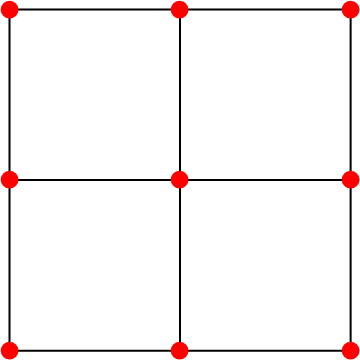
\includegraphics[width=0.2\textwidth]{Sections/Images/SqLattice.png}\ \ \ \ \ \ \ \ \ \ \ \ \ \ 
    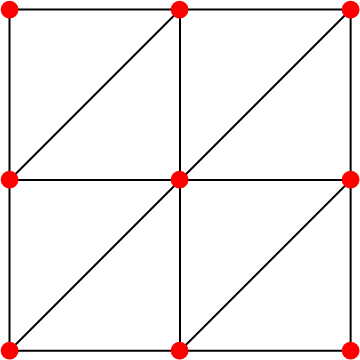
\includegraphics[width=0.2\textwidth]{Sections/Images/TriLattice.png}
    \caption{Связи узлов в квадратной (слева) и треугольной решёток (справа)}
    \label{fig:lattices}
\end{figure}

Между моделями будет проведено сравнение локального координационного числа - средней доли узлов с фиксированным числом соседей $\la n_i \ra$, расчитываемое напрямую как среднее по возможным конформациям отношение мономеров с i соседями к общему количеству узлов в цепочке.

В обоих частях работы нас интересует сравнение поведения описанных моделей в критической области.
В таблицах \ref{tab:Ising_T_c} и \ref{tab:ISAW_T_c}


\begin{table}[h]
    \centering
    \begin{tabular}{|c|c|c|}
        \hline
        Структура & Решётка & $J_{c}$ \\ \hline
        конформация СБС & Квадратная & $0.8340(5)$\cite{faizullina2021critical} \\ \hline
        конформация СБС & 3D-кубическая & $0.5263 \pm 0.055$\cite{foster2021critical}\\ \hline
        регулярная решётка & Прямоугольная & $\ln{(1 + \sqrt{2}) / 2}$\cite{Onsager}\\ \hline
    \end{tabular}
    \caption{Известные значения критической точки $J_c$ некоторых модицикаций модели Ising-ISAW и прямоугольного Изинга}
    \label{tab:Ising_T_c}
\end{table}

\begin{table}[h]
    \centering
    \begin{tabular}{|c|c|}
        \hline
        Решётка & $\beta_{c}$ \\ \hline
        Квадратная & $0.6673(5)$ \cite{caracciolo2011geometrical} \\ \hline
        3D-кубическая & $0.2779 \pm 0.0041$\cite{Tesi1996} \\ \hline
        Треугольная & $ 0.405 \pm 0.07$\cite{Privman1986} \\ \hline
    \end{tabular}
    \caption{Известные значения критической точки $\beta_c$ некоторых модицикаций модели ISAW}
    \label{tab:ISAW_T_c}
\end{table}

Для симуляции моделей в несколькими степенями свобод применяются методы Монте-Карло.
Исследуемая модель Ising-ISAW уже рассматривалась ранее в работах \cite{Garel1999, Papale2018} задаче замороженного беспорядка - когда свойства модели исследовались генерацией спиновой подсистемы на уже сгенерированных конформациях.
В нашей работе исследуется задача динамического беспорядка, в которой генерируются одновременно и блуждания фиксированной длины N, и спиновые состояния на ней.
Для этого используется алгоритм на основе метода Червя (для генерации движущихся конформаций), и кластерного алгоритма Вольфа. 
Для генераций родительских моделей оба метода применяются по отдельности.
Полное описание используемого метода моделирования описаны в работе \cite{faizullina2021critical}.



